%Travail technique
	%But?
	%Overview (Mockups, workflows)
	%Algorithme
	%Architecture et Design
	%Implémentation (langage et librairies utilisés)
	%Utilisation (screenshots, etc)


\chapter{Travail technique}
	\thispagestyle{document}
	
\section{Principe}
\label{sec:principe}
\par Le principe est d'utiliser les suites de tests d'un projet comme spécifications de celui-ci. Ces spécifications contiennent deux types de valeurs très importantes. Premièrement les variables accessibles lors d'un comportement exécuté par l'application : les entrées. Ensuite la valeur attendue de ce comportement : la sortie. De ce fait, OLS-Repair ne dépend pas du type de bug car il considère la méthode défaillante comme une boîte noire. À la manière de Nopol\cite{nopol}, il de suffit trouver une relation entre les entrées et les sorties à l'aide de solver SMT. Cette relation représentera le comportement nominal de l'application et remplacera la boîte noire. Les tests sont ensuite utilisés comme spécifications exécutables pour valider la solution synthétisée.


\section{Overview}
\label{sec:overview}
\begin{figure}[H]
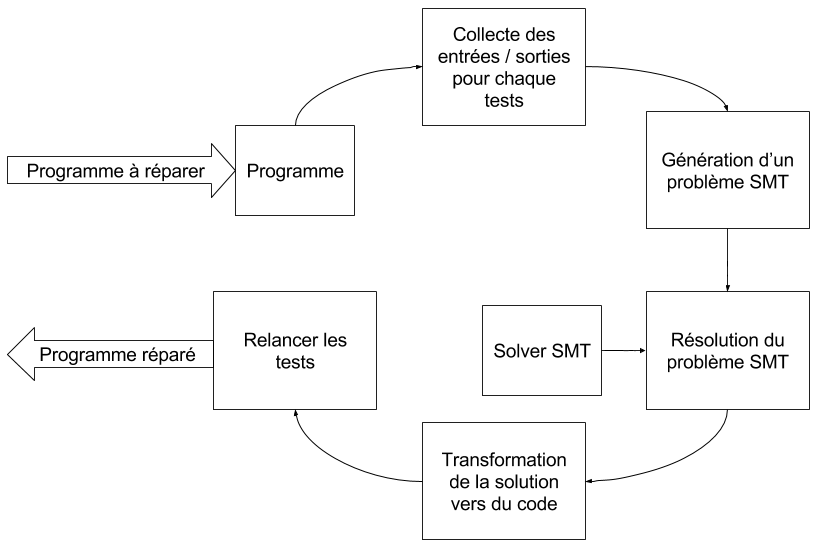
\includegraphics[scale=0.5]{workflowSMT.png}
\caption{Workflow de l'exécution du programme}
\label{fig:workflow}
\end{figure}

\subsection{Collecte}
\label{subsec:collecte}
\par La phase de collecte de données a pour objectif d'obtenir les entrées et la sortie pour chaque tests. Ces entrées / sorties sont vues comment des spécification, elles sont définies de la manière suivante : $S_{i}(I,O)$, où $I$ représente l'ensemble des entrées pour le test $i$, et $O$ la sortie pour le test $i$. 

\subsection{Génération}
\par La phase de génération transforme l'ensemble des spécifications collectées en \ref{subsec:collecte} en un problème SMT en utilisant les mêmes algorithmes que ceux définis dans Nopol\cite{nopol}. Ces algorithmes ajoutent également des constantes à $I$, valeurs souvent utilisées dans des expressions mathématiques, tel que $-1$, $0$ et $1$. 
\subsection{Résolution et synthèse}
\label{subsec:synthese}
\par La phase de résolution est déléguée à un solver SMT. Ce dernier est appelé de manière itérative. Tous d'abord sur un problème avec un nombre d'opérateurs restreints. Ensuite, si le problème n'est pas \textit{décidable}, alors de nouveaux opérateurs sont ajoutés pour augmenter l'espace de recherche. Ces opérateurs sont définis dans la table \ref{table:operators}


\begin{table}[H]
\centering
\begin{tabular}{|c|c|}
  \hline
  Itération & Opérateurs encodés \\
  \hline
  1 & Aucun opérateur  \\
  2 & == != $<$ $<=$   \\
  3 & ! $|$ $|$ \&\&  \\
  4 & + -  \\
  5 & ?  \\
  6 & *  \\
  \hline
\end{tabular}

\caption{Opérateurs encodés en fonction du nombre d'itérations effectuées avec le solver SMT}
\label{table:operators}
\end{table}

\par Lorsque le problème est dit \textit{décidable}, une ligne de code est synthétisée en fonction de la solution proposée par le solver. Cette ligne remplacera ensuite le corps de la méthode contenant le bug.

\subsection{Validation de la synthèse}

\par Les spécifications mentionnées en \ref{subsec:collecte} permettent de valider ou d'invalider la ligne synthétisée. Une fois insérée dans le code source, le code est compilé et les tests sont exécutés pour valider la synthèse.





\section{Scope}
\label{sec:scope}

\subsection{Programmes}

OLS-Repair s'applique uniquement sur des programmes Java. Ces derniers doivent contenir des tests écrits à l'aide du framework JUnit\footnote{\url{http://junit.org/}}.


\subsection{Collecte}

La collecte des spécifications expliquées en \ref{subsec:collecte} est statiques. OLS-Repair collecte uniquement les valeurs des paramètres de méthodes utilisées dans une assertion JUnit.

\subsection{Forme des tests}

Afin de pouvoir collecter de manière statique les paramètres de méthodes, les tests doivent être écrits de la manière présentée dans la figure \ref{fig:forme_collecte}.

\begin{figure}[H]
\begin{lstlisting}
public void test() throws Exception {
    Calculatrice calc = new Calculatrice();
    int expected = 6;
    int a = 2;
    int b = 4;
    Assert.assertEquals(expected, calc.add(a, b));
}
\end{lstlisting}
\caption{Exemple de code permettant à OLS-Repair la collecte des spécifications}
\label{fig:forme_collecte}
\end{figure}


\subsection{Type des entrées / sorties}

OLS-Repair se limite à différents types pour $I$ et $O$. La table \ref{table:IO} représente les types supportés. Afin de  prendre en compte des tableaux, tous ces derniers doivent être de la même taille.

\begin{table}[H]
\centering
\begin{tabular}{|c|c|c|}
  \hline
  Type & $I$ & $O$ \\
  \hline
  int 		& \checkmark & \checkmark \\
  int[] 	& \checkmark & \ding{56} \\
  \hline
\end{tabular}

\caption{Opérateurs encodés en fonction du nombre d'itérations effectuées avec le solver SMT}
\label{table:IO}
\end{table}


\section{Implementation}
\label{sec:implementation}

\par OLS-Repair est implementé en Java. Cette approche utilise Spoon\footnote{\url{http://spoon.gforge.inria.fr/}}, une librairie d'analyses et de transformations de codes sources pour instrumenter les tests, collecter les entrées / sorties et insérer un patch.
\par La transformation des spécifications en problème SMT utilise les algorithmes déjà définis dans Nopol\cite{nopol}. Ces algorithmes utilisent JSMTLIB\footnote{\url{https://github.com/smtlib/jSMTLIB}}, une API permettant la génération de script SMT-LIB\footnote{\url{http://smtlib.cs.uiowa.edu/}}. Ce langage est un standard compréhensible par différents solvers SMT.
\par Le solver utilisé est Z3\footnote{\url{https://z3.codeplex.com/}}, ce solver embarque les théories non-linéaires sur les réels, ce qui le démarque des autres. C'est grâce à Z3 que l'opérateur de multiplication mentionné en \ref{subsec:synthese} peut être utilisé.


\section{Utilisation}

OLS-Repair est paramétrable, il se lance de la manières suivante :
\\
\begin{verbatim}
Usage: OLS_Repair
       -s, --source-path path_buggy_program
       -j, --junit-path path_junit_jar
       -z, --z3-path path_z3_executable
      [-c, --constant one_constant_to_add]*
      [-o, --override]
      [-u, --use-blackbox]
\end{verbatim}


	

	
		
		
		